% Provenance (never printed): see sources/outline_sources.md (Year 2: ancient massifs,
% Caledonian and Variscan belts; the Wilson cycle; supercontinents). Caledonian phases after
% McKerrow, Mac Niocaill and Dewey (2000) and Schiffer et al. (2020); the Wilson cycle after
% Chenin et al. (2018) and Schiffer et al. (2020); the Variscan belt after Faure (2024);
% supercontinents after Nance (2022); Siccar Point after the IUGS Geoheritage description.
% Model ocean and supercontinent chart from figdata/bachelor-2/wilson.py. Exercise and problem
% values in the Book 4 scratch calculator calc/ch15.py.
\chapter{Oude massieven en de Wilsoncyclus}\label{ch:b2:wilson-cycle}

Aan de kust van het zuidoosten van Schotland, bij Siccar Point, staan grijze zandsteenlagen rechtop
onder een kap van rode zandsteen die zacht naar de zee helt. De grijze lagen werden afgezet in
een oceaan vroeg in het Siluur, daarna geplooid en van splijting voorzien toen die oceaan sloot; ze werden
afgesleten tot een oneffen oppervlak; in het Laat-Devoon begroeven rode grindlagen ze, en een tweede,
zachtere gebergtevorming kantelde op haar beurt de rode lagen. Eén klif legt een oceaan vast die
verdwenen is, een gebergtegordel die weg is, en de volgende. Dit hoofdstuk leest zulke archieven,
brengt ze samen in een cyclus die oceaanbekkens volgen, en neemt afstand tot het langste ritme van
alle, het samenvoegen en uiteenvallen van \omterm{def:b2:wilson-cycle:supercontinent}{supercontinenten}.
% ledger: iugs:siccar-orogenies, iugs:siccar-point

\begin{recall}
\textbf{Uit de schoolboeken}: Pangea en het uiteenvallen ervan, \omterm{def:b2:wilson-cycle:supercontinent}{supercontinenten}; discordanties;
de denudatiesnelheid, isostatisch herstel, en het exponentiële verval van een bergketen die door
zijn rivieren wordt afgesleten. \textbf{Uit Boek~3}: continentale riften, passieve randen en
mid-oceanische ruggen, de volledige en de halve spreidingssnelheid; subductie en actieve randen.
\textbf{Uit \cref{ch:b2:crustal-melting} tot \cref{ch:b2:himalaya-andes}}: \omterm{def:b2:crustal-melting:migmatite}{migmatieten} en
granieten; \omterm{def:b2:alpine-orogen:orogen}{orogeen}, \omterm{def:b2:alpine-orogen:ophiolite}{ofioliet}, sutuur, \omterm{def:b2:alpine-orogen:nappes}{dekblad}, \omterm{def:b2:alpine-orogen:foreland}{flysch} en \omterm{def:b2:alpine-orogen:foreland}{molasse}, \omterm{def:b2:alpine-orogen:foreland}{voorlandbekken}; \omterm{def:b2:himalaya-andes:types}{botsingsorogenen} en
\omterm{def:b2:alpine-orogen:orogen}{orogenen} van Andestype; \omterm{def:b2:himalaya-andes:thickening}{korstverdikking}, Airy-dikte en \omterm{def:b2:himalaya-andes:collapse}{gravitationele ineenstorting}.
\end{recall}

\begin{omfigure}
\centering
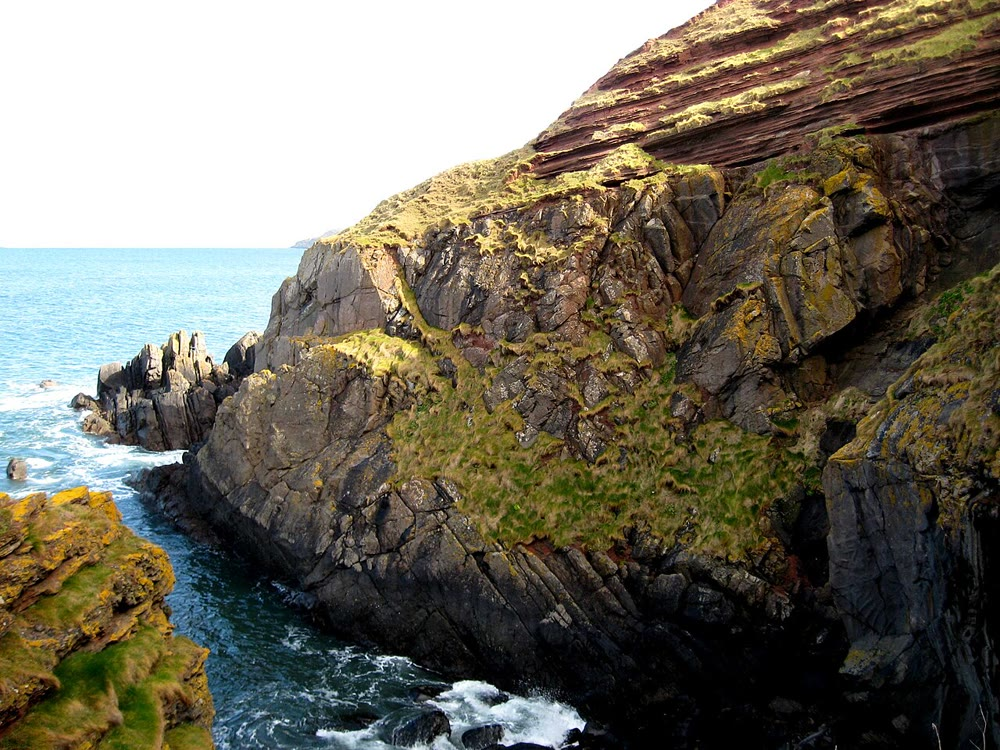
\includegraphics[width=0.64\linewidth]{images/book4/b2-15-siccar-point.jpg}
\par\smallskip{\small Siccar Point, ten zuidoosten van de landtong: bijna verticale lagen grijze
Silurische grauwacke, geplooid in de Caledonische orogenese, onder zacht hellende rode lagen van het
Boven-Devoon. Foto dave souza, 2008, CC BY-SA 4.0.}
\end{omfigure}
% ledger: iugs:siccar-orogenies

\section{Gordels afgesleten tot op hun wortels}\label{sec:b2:wilson-cycle:old}

West-Europa en het oosten van Noord-Amerika worden doorkruist door gebergtegordels die veel ouder zijn dan de
Alpen. Hun toppen zijn verdwenen, maar hun gesteenten blijven. Drie ervan zijn hier van belang.

De \emph{Caledonische} gordel loopt van Noorwegen via Schotland en Ierland naar Newfoundland en
de noordelijke Appalachen, en verder door Oost-Groenland en Spitsbergen. Ze is het archief van een
oceaan, de Iapetus, die in het vroege Paleozoïcum lag tussen Laurentia, de voorouder van
Noord-Amerika en Groenland, in het noordwesten, en Baltica en Avalonia in het zuidoosten en oosten.
Haar randen waren ongeveer 600 miljoen jaar geleden uiteengescheurd; haar sluiting, van het Cambrium tot het
Devoon, bracht een hele reeks botsingen voort, zodat de Caledonische orogenese zo'n
200 miljoen jaar beslaat. De term noemt een plaats en een oceaan, geen ouderdom.
% ledger: mckerrow00:caledonian, schiffer20:caledonides

De \emph{Varistische} gordel, in oudere teksten Hercynisch genoemd, doorkruist Europa vanaf het zuidwesten van
Engeland en België via Frankrijk en Iberië tot in Midden-Europa; de \emph{Appalachische} gordel van
het oosten van Noord-Amerika is zijn westelijke tweeling. Samen leggen ze de sluiting vast van de oceanen
tussen het zuidelijke continent, Gondwana, en het noordelijke, dat net was samengesmeed door
de Caledonische botsingen. Hun laatste botsing, in het Laat-Carboon en Perm, liet
een plooiingsgordel achter die oost--west door Zuid-Europa loopt en noordoost--zuidwest tussen
het oosten van Noord-Amerika en Noordwest-Afrika, en daarmee het \omterm{def:b2:wilson-cycle:supercontinent}{supercontinent} Pangea.
% ledger: schiffer20:variscan, faure24:variscan

Hoe herkent men een gebergtegordel die al driehonderd miljoen jaar wordt geërodeerd?
Niet aan zijn reliëf, dat verdwenen is. Men zoekt zijn onderdelen, die elk in de vorige
hoofdstukken al voorkwamen:
\begin{itemize}
\item \emph{suturen} bezet met \emph{\omterm{def:b2:alpine-orogen:ophiolite}{ofiolieten}}, schijven van de oceaanbodem die sloot;
\item gordels van \emph{metamorfe gesteenten}, vaak van hoge graad, de wortels van de verdikte korst,
nu aan het oppervlak omdat de kilometers erboven zijn geërodeerd;
\item \emph{granieten} en \emph{\omterm{def:b2:crustal-melting:migmatite}{migmatieten}}, de producten van het smelten van de korst dat
verdikking en verhitting meebrengen;
\item sedimenten van de sluitende oceaan en van de gordel: \emph{\omterm{def:b2:alpine-orogen:foreland}{flysch}}, in diepe bekkens afgezet
tijdens de convergentie, \emph{\omterm{def:b2:alpine-orogen:foreland}{molasse}}, in voorland- en intramontane bekkens afgezet;
\item \emph{hoekdiscordanties}, waar jongere lagen rusten op lagen die vóór hen werden geplooid en
geërodeerd, en die de vervorming tussen beide dateren.
\end{itemize}

\begin{definition}[Schiervlakte]\label{def:b2:wilson-cycle:peneplain}
Een \emph{schiervlakte}\index{schiervlakte} (peneplain) is een landoppervlak met gering reliëf, dicht bij het basisniveau van
de erosie, dat door langdurige erosie van een vroeger reliëf over gesteenten van verschillende hardheid en
structuur is gesneden.
\end{definition}

De Varistische gordel is een heet \omterm{def:b2:alpine-orogen:orogen}{orogeen}. In de Alpen van \cref{ch:b2:alpine-orogen} volgden de gesteenten
metamorfe gradiënten van ongeveer \qty{8}{\celsius} per kilometer; in de Varistische gordel
ongeveer \qty{30}{\celsius} per kilometer. Zijn korst smolt op grote schaal: in het Franse Centraal Massief
en het Armoricaans Massief ontstonden \omterm{def:b2:crustal-melting:migmatite}{migmatieten} tussen ongeveer 330 en 325 miljoen jaar geleden, en
granieten drongen erin binnen. Dat smelten is het belangrijkste verschil met de Westelijke Alpen. Toen de
botsing eindigde, werd de verdikte korst door rek dunner, werden metamorfe gesteenten omhooggebracht
langs onthechtingsvlakken, en gingen intramontane bekkens open; daarna vlakte de erosie de keten af tot een
Permische en Triassische \omterm{def:b2:wilson-cycle:peneplain}{schiervlakte} waarop de sedimenten van de volgende cyclus werden afgezet.
% ledger: faure24:variscan

\begin{omfigure}
\centering\small
\begin{tabular}{>{\raggedright\arraybackslash}p{0.2\linewidth}|>{\raggedright\arraybackslash}p{0.17\linewidth}|>{\raggedright\arraybackslash}p{0.52\linewidth}}
fase & ouderdom & wat er botste \\ \hline
Penobscotisch & 490--485 Ma & een eilandboog op de Avalonische rand geschoven \\
Grampisch, Taconisch & 480--455 Ma & eilandbogen tegen Laurentia (Schotland; de noordelijke Appalachen) \\
Shelveisch & vroeg Laat-Ordovicium & Avalonia tegen Baltica; de Tornquistzee sluit \\
Scandisch & 425--400 Ma & Baltica tegen Laurentia; de grote \omterm{def:b2:alpine-orogen:nappes}{dekbladen} van Scandinavië \\
Acadisch & Vroeg-Devoon & \omterm{def:b2:wilson-cycle:terrane}{terranes} uit Gondwana tegen het nieuwe continent; Iapetus gesloten \\
\end{tabular}
\par\smallskip{\small De belangrijkste fasen van de Caledonische orogenese. De vroege fasen zijn
botsingen van bogen met bogen of continenten, de late botsingen van continenten; de meeste
fasen begonnen op verschillende plaatsen op verschillende tijdstippen.}
\end{omfigure}
% ledger: mckerrow00:phases, schiffer20:caledonides

De Caledonische tabel hierboven toont het andere kenmerk van oude gordels: ze zijn samengesteld. Voordat de
twee continenten elkaar ontmoetten, kwamen bogen en kleinere blokken een voor een aan en werden ze vastgesmeed.

\begin{definition}[Terrane; microcontinent]\label{def:b2:wilson-cycle:terrane}
Een \emph{terrane}\index{terrane} is een door breuken begrensd korstblok waarvan de geologische geschiedenis
verschilt van die van zijn buren, door plaatbeweging naar zijn huidige positie gebracht; het kan
een eilandboog, een oceanisch plateau, een schijf oceaanbodem of een fragment van een continent zijn. Een
\emph{microcontinent}\index{microcontinent} is een blok continentale korst, kleiner dan een
continent, dat door oceanische korst van de continenten is gescheiden.
\end{definition}

Avalonia was zo'n blok: een strook korst die de rand van Gondwana verliet, achter zich in het Ordovicium de Rheïsche
Oceaan opende, de Iapetus overstak en aanmeerde tegen Baltica en daarna
Laurentia. Armorica en Saxothuringia, nu in Frankrijk en Duitsland, volgden het op hun beurt; hun
suturen, gemarkeerd door \omterm{def:b2:alpine-orogen:ophiolite}{ofiolieten}, verdelen de Varistische gordel in zones van een noordelijk voorland
in het oude noordelijke continent tot een zuidelijk voorland in Gondwana.
% ledger: schiffer20:caledonides, schiffer20:variscan, faure24:variscan

\begin{omfigure}
\centering
\begin{tikzpicture}[x=0.5cm, y=0.5cm, font=\scriptsize]
\tikzset{cont/.style={fill=orange!25, draw=black!60, line width=0.4pt},
  terr/.style={fill=orange!45, draw=black!60, line width=0.4pt},
  ocn/.style={font=\scriptsize\itshape, text=blue!50!black},
  belt/.style={pattern=north east lines, pattern color=red!60!black, draw=red!60!black}}
% panel A
\begin{scope}
\fill[blue!6] (0,0) rectangle (9,8);
\draw[cont] (0.3,4.2) -- (3.0,4.0) -- (3.4,7.7) -- (0.3,7.7) -- cycle;
\node[align=center] at (1.7,6.0) {Lau-\\rentia};
\draw[cont] (6.0,5.4) -- (8.7,5.0) -- (8.7,7.7) -- (6.4,7.7) -- cycle;
\node at (7.4,6.6) {Baltica};
\draw[cont] (0.3,0.3) -- (8.7,0.3) -- (8.7,1.6) -- (0.3,1.9) -- cycle;
\node at (4.5,0.95) {Gondwana};
\draw[terr] (3.8,2.4) -- (6.6,2.2) -- (6.6,2.9) -- (3.8,3.1) -- cycle;
\node at (5.2,2.65) {Avalonia};
\node[ocn] at (4.6,5.4) {Iapetus};
\node[ocn] at (7.7,2.55) {Rheïsch};
\node[anchor=north west, font=\small\bfseries] at (0.1,8.9) {A: ongeveer 480 Ma};
\end{scope}
% panel B
\begin{scope}[xshift=5.0cm]
\fill[blue!6] (0,0) rectangle (9,8);
\draw[cont] (0.3,3.6) -- (3.0,3.4) -- (3.4,7.7) -- (0.3,7.7) -- cycle;
\draw[cont] (3.0,3.4) -- (3.4,7.7) -- (8.7,7.7) -- (8.7,4.4) -- (5.2,4.6) -- (5.0,3.4) -- cycle;
\draw[terr] (3.0,3.4) -- (5.0,3.4) -- (5.2,4.6) -- (8.7,4.4) -- (8.7,3.6) -- (3.0,2.8) -- cycle;
\draw[red!60!black, line width=1.2pt] (3.0,3.4) -- (3.4,7.7);
\draw[red!60!black, line width=1.2pt] (5.0,3.4) -- (5.2,4.6) -- (8.7,4.4);
\node[align=center] at (1.6,5.6) {Lau-\\rentia};
\node at (6.6,5.7) {Baltica};
\node at (6.4,3.75) {Avalonia};
\node at (6.0,7.1) {\textbf{Laurussia}};
\draw[cont] (0.3,0.3) -- (8.7,0.3) -- (8.7,1.3) -- (0.3,1.5) -- cycle;
\node at (4.5,0.8) {Gondwana};
\draw[terr] (2.2,1.9) -- (3.6,1.9) -- (3.6,2.3) -- (2.2,2.3) -- cycle;
\draw[terr] (5.0,1.8) -- (6.6,1.8) -- (6.6,2.2) -- (5.0,2.2) -- cycle;
\node[ocn] at (7.7,2.3) {Rheïsch};
\node[anchor=north west, font=\small\bfseries] at (0.1,8.9) {B: ongeveer 420 Ma};
\end{scope}
% panel C
\begin{scope}[xshift=10.0cm]
\fill[blue!6] (0,0) rectangle (9,8);
\draw[cont] (0.3,3.0) -- (8.7,3.0) -- (8.7,7.7) -- (0.3,7.7) -- cycle;
\draw[cont] (0.3,0.3) -- (8.7,0.3) -- (8.7,3.0) -- (0.3,3.0) -- cycle;
\fill[belt] (0.3,2.5) -- (8.7,2.5) -- (8.7,3.5) -- (0.3,3.5) -- cycle;
\node[fill=orange!25, inner sep=1pt] at (4.5,5.6) {Laurussia};
\node[fill=orange!25, inner sep=1pt] at (4.5,1.3) {Gondwana};
\node[fill=white, fill opacity=0.85, text opacity=1, inner sep=1pt, align=center] at (4.5,3.0)
  {Varistisch-Appalachische gordel};
\node[ocn] at (7.6,0.7) {};
\node[anchor=north west, font=\small\bfseries] at (0.1,8.9) {C: ongeveer 300 Ma, Pangea};
\end{scope}
\end{tikzpicture}
\par\smallskip{\small Drie momenten van de sluiting van de Iapetus en de Rheïsche Oceaan, als een
schematische schets zonder kaartprojectie en zonder schaal: posities, groottes en vormen zijn alleen
topologisch. A: Avalonia heeft Gondwana verlaten en de Rheïsche Oceaan gaat erachter open. B: Iapetus is
gesloten; Laurentia, Baltica en Avalonia vormen Laurussia, langs Caledonische suturen (rode lijnen);
kleinere blokken steken de Rheïsche Oceaan over. C: Gondwana heeft Laurussia ontmoet langs de
Varistisch-Appalachische gordel (gearceerd).}
\end{omfigure}
% ledger: mckerrow00:caledonian, mckerrow00:phases, schiffer20:caledonides, schiffer20:variscan, faure24:variscan

\section{De Wilsoncyclus}\label{sec:b2:wilson-cycle:cycle}

In 1966 vroeg J. Tuzo Wilson zich af of de Atlantische Oceaan gesloten was en daarna
weer opengegaan. Fossielen uit het vroege en midden-Paleozoïcum vertelden hem dat een wijde oceaan toen
de fauna's van Noord-Amerika had gescheiden van die van West-Europa, een oceaan die niet meer
bestond van het late Paleozoïcum tot het midden van het Mesozoïcum. De moderne Atlantische Oceaan was opengegaan
bijna waar die oudere oceaan, de Iapetus, was gesloten.
% ledger: schiffer20:wilson, chenin18:cycle

\begin{definition}[Wilsoncyclus]\label{def:b2:wilson-cycle:wilson}
De \emph{Wilsoncyclus}\index{Wilsoncyclus} is de opeenvolging van stadia waarin een
oceaanbekken tussen continentale randen opengaat en weer sluit: continentale riftvorming,
opbreken en oceaanbodemspreiding, een wijder wordende oceaan met passieve randen, het begin van
subductie, het versmallen en sluiten van de oceaan, continentale botsing, en de ineenstorting
en erosie van de gordel, waarna het samengesmede continent langs dezelfde zone opnieuw kan uiteenscheuren.
\end{definition}

De figuur hieronder volgt de stadia. Het zijn die van de vorige hoofdstukken, in volgorde gezet:
de riften en passieve randen uit Boek~3, de actieve randen en hun bogen, de
Alpiene en Himalaya-botsingen, de \omterm{def:b2:himalaya-andes:collapse}{gravitationele ineenstorting} van Tibet, het trage afslijten
van de oude gordels.

\begin{omfigure}
\centering
\begin{tikzpicture}[x=0.38cm, y=0.38cm, font=\scriptsize]
\tikzset{crust/.style={fill=orange!25, draw=black!60, line width=0.3pt},
  ocrust/.style={fill=gray!45, draw=black!60, line width=0.3pt},
  sea/.style={fill=blue!8},
  ttl/.style={anchor=west, font=\scriptsize\bfseries}}
% 1 continent
\begin{scope}
\draw[crust] (0,0) -- (16,0) -- (16,2) -- (0,2) -- cycle;
\node[ttl] at (0,3.1) {1\enspace een continent};
\end{scope}
% 2 rift
\begin{scope}[xshift=7.2cm]
\draw[crust] (0,0) -- (7,0) -- (7,2) -- (6.2,2) -- (5.4,1.0) -- (0,2) -- cycle;
\draw[crust] (9,0) -- (16,0) -- (16,2) -- (10.6,1.0) -- (9.8,2) -- (9,2) -- cycle;
\fill[red!50] (7,0) -- (9,0) -- (8.6,1.2) -- (7.4,1.2) -- cycle;
\draw[thick] (6.2,2) -- (7,0.4); \draw[thick] (9.8,2) -- (9,0.4);
\node[ttl] at (0,3.1) {2\enspace rift};
\end{scope}
% 3 young ocean
\begin{scope}[yshift=-2.4cm]
\fill[sea] (5,2) -- (11,2) -- (11,0.6) -- (5,0.6) -- cycle;
\draw[crust] (0,0) -- (5,0) -- (6.2,0.5) -- (5,2) -- (0,2) -- cycle;
\draw[crust] (16,0) -- (11,0) -- (9.8,0.5) -- (11,2) -- (16,2) -- cycle;
\draw[ocrust] (6.2,0.5) -- (9.8,0.5) -- (9.8,0) -- (6.2,0) -- cycle;
\draw[red!70!black, thick] (8,0.5) -- (8,1.0);
\node[ttl] at (0,3.1) {3\enspace een jonge oceaan};
\end{scope}
% 4 wide ocean
\begin{scope}[xshift=7.2cm, yshift=-2.4cm]
\fill[sea] (2.5,2) -- (13.5,2) -- (13.5,0.4) -- (2.5,0.4) -- cycle;
\draw[crust] (0,0) -- (2.5,0) -- (3.4,0.4) -- (2.5,2) -- (0,2) -- cycle;
\draw[crust] (16,0) -- (13.5,0) -- (12.6,0.4) -- (13.5,2) -- (16,2) -- cycle;
\draw[ocrust] (3.4,0.4) -- (12.6,0.4) -- (12.6,-0.4) -- (3.4,-0.4) -- cycle;
\draw[red!70!black, thick] (8,0.4) -- (8,0.9);
\node[anchor=north] at (3,-0.1) {passief};
\node[anchor=north] at (13,-0.1) {passief};
\node[ttl] at (0,3.1) {4\enspace een wijde oceaan};
\end{scope}
% 5 subduction begins
\begin{scope}[yshift=-4.8cm]
\fill[sea] (2.5,2) -- (13.5,2) -- (13.5,0.4) -- (2.5,0.4) -- cycle;
\draw[crust] (0,0) -- (2.5,0) -- (3.4,0.4) -- (2.5,2) -- (0,2) -- cycle;
\draw[crust] (16,-0.4) -- (13.3,-0.4) -- (12.6,0.4) -- (13.5,2) -- (16,2) -- cycle;
\draw[ocrust] (3.4,0.4) -- (12.6,0.4) -- (11.6,-1.6) -- (3.4,-0.4) -- cycle;
\fill[red!60!black] (14.2,2) -- (14.6,2.7) -- (15.0,2) -- cycle;
\draw[red!70!black, thick] (7,0.4) -- (7,0.9);
\node[anchor=north] at (13.5,-0.5) {trog};
\node[ttl] at (0,3.1) {5\enspace subductie begint};
\end{scope}
% 6 ocean closes
\begin{scope}[xshift=7.2cm, yshift=-4.8cm]
\fill[sea] (5.5,2) -- (10.5,2) -- (10.5,0.4) -- (5.5,0.4) -- cycle;
\draw[crust] (0,0) -- (5.5,0) -- (6.4,0.4) -- (5.5,2) -- (0,2) -- cycle;
\draw[crust] (16,-0.4) -- (11.3,-0.4) -- (10.6,0.4) -- (11.5,2.4) -- (16,2.4) -- cycle;
\draw[ocrust] (6.4,0.4) -- (10.6,0.4) -- (9.4,-1.8) -- (6.4,-0.4) -- cycle;
\fill[red!60!black] (12.4,2.4) -- (12.8,3.1) -- (13.2,2.4) -- cycle;
\node[anchor=north west] at (11.6,-0.5) {boog, trog};
\node[ttl] at (0,3.1) {6\enspace de oceaan sluit};
\end{scope}
% 7 collision
\begin{scope}[yshift=-7.2cm]
\draw[crust] (0,0) -- (16,0) -- (16,2) -- (10,2) -- (8.6,3.6) -- (7.4,3.4) -- (6,2) -- (0,2) -- cycle;
\fill[crust] (5.6,0) -- (10.4,0) -- (9.6,-1.6) -- (6.4,-1.6) -- cycle;
\draw[black!60, line width=0.3pt] (5.6,0) -- (6.4,-1.6) -- (9.6,-1.6) -- (10.4,0);
\draw[red!60!black, line width=1pt] (8.6,3.6) -- (7.6,-1.6);
\node[anchor=west, text=red!60!black] at (9.0,3.5) {sutuur};
\node[ttl] at (0,3.1) {7\enspace botsing};
\end{scope}
% 8 worn flat
\begin{scope}[xshift=7.2cm, yshift=-7.2cm]
\draw[crust] (0,0) -- (16,0) -- (16,2) -- (0,2) -- cycle;
\draw[red!60!black, line width=1pt] (8.4,2) -- (7.6,0);
\fill[pink!60!red!40] (6.0,1.0) ellipse (0.7 and 0.4);
\node[anchor=north] at (8,-0.1) {schiervlakte boven de oude wortel};
\node[ttl] at (0,3.1) {8\enspace een afgevlakte gordel; riftvorming kan volgen};
\end{scope}
\end{tikzpicture}
\par\smallskip{\small De stadia van de \omterm{def:b2:wilson-cycle:wilson}{Wilsoncyclus}, als schematische doorsneden (niet op schaal):
continentale korst in oranje, oceanische korst in grijs, de rug in rood, vulkanen van de boog als
driehoekjes; in het laatste paneel blijven de sutuur en een graniet over in een korst van normale dikte.}
\end{omfigure}
% ledger: chenin18:cycle, schiffer20:wilson

\subsection{Hoe breed, hoe lang?}

Een oceaan groeit door oceaanbodemspreiding aan zijn rug en krimpt door subductie aan zijn troggen.
Een eenvoudige boekhouding geeft zijn breedte.

\begin{proposition}[Breedte van een oceaan gedurende een cyclus]\label{prop:b2:wilson-cycle:width}
Laat een oceaan opengaan op tijdstip $t_0$ en wijder worden met de volledige spreidingssnelheid $V_s$ van zijn rug, tot een
subductiezone op tijdstip $t_1$ aan een van de randen begint en oceaanbodem verbruikt met de snelheid $V_c$
ten opzichte van die rand, met $V_c > V_s$, terwijl de rug blijft spreiden. Zijn breedte is
\[
  W(t) = V_s\,(t - t_0) \quad (t_0 \le t \le t_1), \qquad
  W(t) = V_s\,(t_1 - t_0) - (V_c - V_s)\,(t - t_1) \quad (t \ge t_1),
\]
het grootst op $t_1$, en de oceaan sluit een tijd $V_s(t_1 - t_0)/(V_c - V_s)$ nadat de subductie
begint. Bij symmetrische spreiding beweegt de rug naar de trog met $V_c - V_s/2$.
\end{proposition}

\begin{proof}
Houd de rand met de trog vast. Vóór $t_1$ gaan de twee randen uiteen met de volledige
spreidingssnelheid $V_s$, zodat de breedte vanaf nul groeit met $V_s$. Na $t_1$ beweegt de plaat tussen
trog en rug naar de trog met $V_c$; de rug voegt $V_s$ toe aan de afstand
tussen die plaat en de verre plaat, zodat de verre rand naar de trog beweegt met $V_c - V_s$,
de snelheid waarmee de breedte afneemt. De breedte bereikt nul na $V_s(t_1 - t_0)/(V_c -
V_s)$. Bij symmetrische spreiding beweegt de rug met het gemiddelde van de snelheden van de platen aan
weerszijden, $(V_c + (V_c - V_s))/2 = V_c - V_s/2$.
\end{proof}

De figuur hieronder speelt deze boekhouding door voor een modeloceaan van het Iapetustype: spreiding vanaf
\qty{570}{Ma} met \qty{30}{mm} per jaar, subductie vanaf \qty{490}{Ma} die \qty{60}{mm} per
jaar verbruikt. De snelheden zijn aannamen, ronde waarden van de grootte die vandaag in de oceanen wordt gemeten; de
echte Iapetus was noch zo eenvoudig noch zo goed bekend. De modeloceaan bereikt \qty{2400}{km}
en sluit op \qty{410}{Ma}, binnen het tijdsbestek van de Scandische botsing.
% values (wilson.py): max_width_km 2400, closure_Ma 410; ledger: mckerrow00:caledonian, schiffer20:caledonides

\begin{omfigure}
\centering
% figdata/bachelor-2/wilson.py part ocean (model values: assumptions)
\begin{tikzpicture}
\begin{axis}[width=0.8\linewidth, height=5.0cm, x dir=reverse, xmin=360, xmax=600, ymin=0,
  ymax=3300, ytick={0,1000,2000,3000}, xlabel={ouderdom (\unit{Ma})}, ylabel={breedte van de oceaan (\unit{km})},
  tick label style={font=\scriptsize}, label style={font=\small}, xtick={600,560,...,360}]
\addplot[omThm, line width=1.2pt] table[x=t_Ma, y=width_km] {figdata/out/bachelor-2-wilson-ocean.dat};
\draw[dashed, black!50] (axis cs:490,0) -- (axis cs:490,2400);
\draw[dashed, black!50] (axis cs:570,0) -- (axis cs:570,2750);
\draw[dashed, black!50] (axis cs:410,0) -- (axis cs:410,2750);
\node[font=\scriptsize, anchor=south] at (axis cs:570,2750) {spreiding begint};
\node[font=\scriptsize, anchor=south west] at (axis cs:488,2400) {subductie begint};
\node[font=\scriptsize, anchor=south] at (axis cs:410,2750) {botsing};
\node[font=\scriptsize, anchor=west] at (axis cs:540,600) {opengaan met $V_s$};
\node[font=\scriptsize, anchor=south west, align=left] at (axis cs:446,1150) {sluiten\\met $V_c - V_s$};
\end{axis}
\end{tikzpicture}
\par\smallskip{\small Breedte van een modeloceaan gedurende één \omterm{def:b2:wilson-cycle:wilson}{Wilsoncyclus}, volgens
\cref{prop:b2:wilson-cycle:width} met $V_s = \qty{30}{mm}$ per jaar vanaf \qty{570}{Ma} en $V_c
= \qty{60}{mm}$ per jaar vanaf \qty{490}{Ma}. De tijd loopt van links naar rechts.}
\end{omfigure}

\subsection{Opengaan waar het sloot}

Het idee van Wilson berust op een mechanisch idee: een oude gordel is een zwakke zone, en een continent dat
uit elkaar wordt getrokken, breekt bij voorkeur langs zijn zwakke zones in plaats van door zijn sterke, stabiele
binnenste.

\begin{definition}[Structurele reactivering]\label{def:b2:wilson-cycle:reactivation}
De \emph{structurele reactivering}\index{structurele reactivering} van een bestaande structuur
(een breuk, een schuifzone, een sutuur, een lithologisch contact) is de hernieuwde concentratie van
vervorming erlangs, onder een later spanningsveld dat kan verschillen van het veld dat haar vormde.
\end{definition}

De Noord-Atlantische Oceaan is het testgeval, en hij slaagt maar gedeeltelijk. In de Centrale Atlantische Oceaan volgt de
jonge oceaan de Appalachen op de voet. Tussen Scandinavië en Groenland volgt het opbreken
grofweg de Caledonische gordel. Verder naar het zuiden niet: de Iapetus-sutuur loopt nog steeds
door Noord-Engeland en Midden-Ierland, en de Atlantische Oceaan ging ten westen ervan open, waarbij
stukken van de oude korst van Laurentia op de noordwestelijke rand van Europa achterbleven, rond Rockall en Hatton.
Verder naar het noordwesten snijden de Labradorzee en de Baffinbaai dwars door oudere cratons en
gordels. Oude structuren leiden latere riften, maar niet altijd: een zwakte die meer dan 30 tot 50 miljoen jaar
is afgekoeld, kan sterk zijn geworden, en een nieuwe rift kan het diepere
maaksel van de mantel volgen in plaats van de sutuur in de korst. De \omterm{def:b2:wilson-cycle:wilson}{Wilsoncyclus} is een leidraad, geen wet.
% ledger: schiffer20:wilson, schiffer20:reactivation

Niet elke cyclus opent een wijde oceaan. Veel \omterm{def:b2:alpine-orogen:orogen}{orogenen} sluiten embryonale oceanen, riften die nauwelijks
waren beginnen te spreiden, minder dan ongeveer \qty{500}{km} breed: de Alpen, de Pyreneeën, het grootste deel van de
Varistische gordel van West-Europa. Andere sluiten wijde, volwassen oceanen, zoals de Scandinavische
Caledoniden deden. Het verschil blijkt aan het eind. Een gordel die een wijde oceaan sloot, droeg een
langlevende boog, die de mantel eronder van zijn smeltbaar deel beroofde; zijn ineenstorting was arm aan
\omterm{def:b2:magma-emplacement:magma}{magma}, zoals in de Caledoniden. Een gordel die een smal bekken sloot, rust op vruchtbare mantel; zijn
ineenstorting kan rijk zijn aan \omterm{def:b2:magma-emplacement:magma}{magma}, zoals in de Varistische gordel, waar de Moho nu vlak is en de
onderkorst gelaagd, gelezen als basalt dat door onderplating onder de korst is geplaatst of als onderkorst die in hete toestand
is geschoven. Binnen enkele tientallen miljoenen jaren vervagen de
warmteanomalieën van een gordel; zijn structuren blijven.
% ledger: chenin18:cycle

\section{Supercontinenten}\label{sec:b2:wilson-cycle:supercontinents}

\begin{definition}[Supercontinent; supercontinentcyclus]\label{def:b2:wilson-cycle:supercontinent}
Een \emph{supercontinent}\index{supercontinent} is een landmassa die het grootste deel van de continentale
korst van de Aarde in één blok verzamelt. De \emph{supercontinentcyclus}\index{supercontinentcyclus} is het
episodische samenvoegen van de continenten tot een supercontinent en het latere
uiteenvallen ervan, herhaald in de loop van de geschiedenis van de Aarde.
\end{definition}

Pangea, dat Wegener reconstrueerde en de schoolboeken beschreven, bestond van ongeveer 325
tot 200 miljoen jaar geleden. Eerdere \omterm{def:b2:wilson-cycle:supercontinent}{supercontinenten} zijn voorgesteld: Pannotia, ongeveer 620 tot
580 miljoen jaar geleden, waarvan het bestaan omstreden is; Rodinia, ongeveer 950 tot 800 miljoen jaar geleden;
Nuna, ook Columbia genoemd, ongeveer 1.6 tot 1.4 miljard jaar geleden; en, twijfelachtiger, Kenorland,
ongeveer 2.7 tot 2.5 miljard jaar geleden, en Ur, ongeveer 3.0 miljard jaar geleden. Ze lijken
zich te hebben samengevoegd en opgesplitst met tussenpozen van ruwweg een half miljard jaar, sinds misschien het late
Archaïcum. De cyclus is in verband gebracht met de tijdperken van gebergtevorming, met pieken in de ouderdommen van
granieten en van de zirkoonkorrels die ze bevatten, met de groei van de korst, met grote magmatische
provincies, met de zeespiegel en met het klimaat: het samenvoegen van een \omterm{def:b2:wilson-cycle:supercontinent}{supercontinent} valt vaak samen
met afkoeling.
% ledger: nance22:supercontinents

\begin{omfigure}
\centering
% figdata/bachelor-2/wilson.py part supercontinents; ledger: nance22:supercontinents
\begin{tikzpicture}
\begin{axis}[width=0.86\linewidth, height=4.6cm, x dir=reverse, xmin=0, xmax=3300, ymin=-0.7,
  ymax=6.5, ytick=\empty, xlabel={ouderdom (\unit{Ma})}, tick label style={font=\scriptsize},
  label style={font=\small}, xtick={0,500,...,3000}, axis y line*=left,
  % namen: expliciete knopen (de figdata-tabel bevat de Engelse namen)
  clip=false]
\addplot[only marks, mark=*, mark size=1.6pt, omThm,
  error bars/.cd, x dir=both, x explicit, error bar style={line width=3pt, omThm!60}, error mark=none]
  table[x=mid_Ma, y=row, x error=half_Ma] {figdata/out/bachelor-2-wilson-supercontinents.dat}; \foreach \x/\y/\n in {3000/0/Ur, 2600/1/Kenorland, 1500/2/Nuna-Columbia, 875/3/Rodinia, 600/4/Pannotia, 262.5/5/Pangea} {\edef\temp{\noexpand\node[font=\noexpand\scriptsize, anchor=south, yshift=2pt] at (axis cs:\x,\y) {\n};}\temp}
\end{axis}
\end{tikzpicture}
\par\smallskip{\small \omterm{def:b2:wilson-cycle:supercontinent}{Supercontinenten} in de loop van de geschiedenis van de Aarde, van samenvoeging tot uiteenvallen, zoals
gedateerd in een recent overzicht: de balken overspannen de opgegeven intervallen (voor Ur is er één schatting), de
stippen hun middens. Pannotia, Kenorland en Ur zijn omstreden. De tijd loopt van links naar rechts.}
\end{omfigure}

Is de cyclus werkelijk periodiek? De middens van de intervallen in de grafiek liggen 400,
1100, 625, 275 en 337.5 miljoen jaar uit elkaar: gemiddeld ongeveer 550, maar verspreid over een factor
vier. ``Ruwweg een half miljard jaar'' is een tendens, geen klok, en de vroegere
\omterm{def:b2:wilson-cycle:supercontinent}{supercontinenten} berusten op schaarse aanwijzingen.
% values (wilson.py): spacings 400 1100 625 275 337.5, mean 547.5 Myr

\section{Van bergen tot vlakten}\label{sec:b2:wilson-cycle:erosion}

Wat maakt van een gordel als de Himalaya de lage heuvels van Bretagne? Boek~2
bouwde een model: rivieren slijten een keten af met een snelheid evenredig met haar gemiddelde hoogte, $kh$,
en elke meter die van de top wordt verwijderd, wordt deels teruggegeven door isostatisch herstel, zodat slechts
de fractie $f = (\rho_m - \rho_c)/\rho_m$ ervan als hoogte verloren gaat. De gemiddelde hoogte
neemt dan af als
\[
  h(t) = h_0\,e^{-k f t} ,
\]
met de tijdconstante $\tau = 1/(kf)$. In grote stroomgebieden op middelbare breedte is de denudatiesnelheid
evenredig met het gemiddelde reliëf, en zonder opheffing zou het reliëf tot een tiende van zijn
waarde dalen in ongeveer 11 miljoen jaar: $k = \ln 10/11 \approx 0.21$ per miljoen jaar. Met de
dichtheden 2700 en \qty{3300}{kg.m^{-3}} is $f = 0.18$ en $\tau \approx \qty{26}{Myr}$: een
keten van \qty{3}{km} hoog staat zo'n 30 miljoen jaar later nog \qty{1}{km} hoog, en zakt
onder \qty{300}{m} na ongeveer 60 miljoen jaar.
% ledger: ahnert70:decay; values (wilson.py): k 0.20933 /Myr, f 0.18182, tau 26.275 Myr

Hetzelfde herstel verklaart waarom oude gordels hun wortels blootleggen. Om een korst die van
$H$ tot $T$ is verdikt terug te brengen tot zeeniveau, moet de hele extra dikte $T - H$ worden geërodeerd, terwijl de gemiddelde
hoogte slechts $(T - H)f$ was: er wordt ongeveer 5.5 keer meer gesteente verwijderd dan de hoogte van de
keten. Gesteenten die 20 of \qty{30}{km} diep in de wortel zaten, komen aan het oppervlak: de
\omterm{def:b2:crustal-melting:migmatite}{migmatieten}, granieten en hooggradige gneisen van de oude massieven, zoals die van het Centraal
Massief.
% ledger: ahnert70:decay

De Varistische keten, waarvan de laatste botsingen ongeveer 290 miljoen jaar geleden eindigden, was
tijdens het Perm en Trias tot een \omterm{def:b2:wilson-cycle:peneplain}{schiervlakte} afgevlakt: binnen de ongeveer 60 miljoen jaar
die het model geeft. Ineenstorting kan het sneller maken: de rek van een verdikte korst, zoals in
Tibet vandaag, maakt die rechtstreeks dunner, zonder op de rivieren te wachten. En bij Siccar Point rusten grindlagen uit het Laat-Devoon op
Silurische lagen die in de Caledonische botsingen zijn geplooid, op een oud landoppervlak dat nog
wat reliëf bewaart tussen de harde en de zachte lagen.
% ledger: faure24:variscan, iugs:siccar-orogenies

\begin{inthefield}[Een hoekdiscordantie lezen]
Geologen die een hoekdiscordantie zoals Siccar Point bestuderen, beginnen met het meten van de
stand van de lagen onder en boven het vlak, strekking en helling, op veel plaatsen. Ze zoeken
de bovenkant van de onderste lagen, aan gradatiegelaagdheid of aan de sporen op de onderkant van de lagen,
omdat geplooide lagen omgekeerd kunnen liggen. Ze onderzoeken het vlak zelf: zijn reliëf, de
verwering eronder, de keien van de oudere gesteenten in het conglomeraat erboven. Daarna
dateren ze: de jongste fossielen eronder geven de ouderdom waarvóór de plooiing niet kan hebben plaatsgevonden,
de oudste fossielen erboven de ouderdom waarvóór ze had plaatsgevonden en het land was afgesleten.
Het interval tussen beide omsluit de orogenese. Bij Siccar Point zijn de onderste lagen
vroeg-Silurisch en de bovenste uit het Laat-Devoon, en de Caledonische plooiing, opheffing en erosie passen
ertussen; de zachte kanteling van de bovenste lagen is nog jonger, Varistisch.
\end{inthefield}
% ledger: iugs:siccar-orogenies, ics:base.Silurian, ics:base.Devonian, ics:base.Carboniferous

\section*{Oefeningen}\label{sec:b2:wilson-cycle:exercises}

Gegevens voor de oefeningen: $g = \qty{9.8}{m.s^{-2}}$; dichtheden van korst en mantel
\qty{2700}{kg.m^{-3}} en \qty{3300}{kg.m^{-3}}; normale korst $H = \qty{35}{km}$; ouderdommen van de
basis van het Siluur, Devoon en Carboon 443.1, 419.6 en \qty{358.9}{Ma}, van het
Trias \qty{251.9}{Ma}.

\begin{exercise}[$\star$]\label{exo:b2:wilson-cycle:1}
De randen van de Iapetus scheurden uiteen rond \qty{600}{Ma}; de belangrijkste Caledonische botsing, de
Scandische, eindigde rond \qty{400}{Ma}; de eerste botsing van een boog met Laurentia begon
rond \qty{480}{Ma}. (a) Hoe lang duurde de hele cyclus van de Iapetus? (b) Hoe lang duurden de
botsingen? (c) Waarom mag ``Caledonisch'' niet worden gebruikt om een ouderdom aan te duiden?
\end{exercise}

\begin{exercise}[$\star$]\label{exo:b2:wilson-cycle:2}
Zet deze situaties in de volgorde van de \omterm{def:b2:wilson-cycle:wilson}{Wilsoncyclus} en benoem het stadium van elk: (a) de
Rode Zee, een smalle oceaan tussen jonge uiteengescheurde randen; (b) de Himalaya; (c) de Oost-Afrikaanse
rift; (d) de Atlantische Oceaan, wijd, met passieve randen aan beide kanten; (e) de Pacifische rand
van Zuid-Amerika; (f) de lage heuvels van Bretagne op een oude sokkel van graniet en gneis.
\end{exercise}

\begin{exercise}[$\star$]\label{exo:b2:wilson-cycle:3}
Bij Siccar Point liggen vroeg-Silurische lagen onder lagen uit het Laat-Devoon. (a) Tussen welke grenzen,
gegeven door de gegevens hierboven, moeten de plooiing, opheffing en erosie hebben plaatsgevonden? (b) Wat is
de langste tijd die ze kunnen hebben geduurd? (c) Som in volgorde de gebeurtenissen op die de klif vastlegt.
\end{exercise}

\begin{exercise}[$\star$]\label{exo:b2:wilson-cycle:4}
Zeg of elk een \omterm{def:b2:wilson-cycle:terrane}{terrane}, een \omterm{def:b2:wilson-cycle:terrane}{microcontinent}, beide of geen van beide is, en waarom: (a) Avalonia;
(b) Laurentia; (c) een eilandboog die aan een continent is vastgegroeid; (d) de Iapetus-sutuur.
\end{exercise}

\begin{exercise}[$\star\star$]\label{exo:b2:wilson-cycle:5}
Neem de middens van de intervallen van de \omterm{def:b2:wilson-cycle:supercontinent}{supercontinenten} Ur (3000), Kenorland (2600),
Nuna (1500), Rodinia (875), Pannotia (600) en Pangea (262.5), in miljoenen jaren geleden.
(a) Bereken de vijf tussenafstanden en hun gemiddelde. (b) Wat is de verhouding van de grootste tussenafstand tot
de kleinste? (c) Laat Kenorland en Ur weg, die twijfelachtig zijn: wat is de gemiddelde tussenafstand van de
andere vier? Is ``een half miljard jaar'' een periode?
\end{exercise}

\begin{exercise}[$\star\star$]\label{exo:b2:wilson-cycle:6}
Een oceaan van \qty{3000}{km} breed begint aan een van zijn randen te worden gesubduceerd met \qty{70}{mm} per jaar,
terwijl zijn rug spreidt met \qty{25}{mm} per jaar. (a) Hoe lang duurt het voordat hij sluit?
(b) Hoe lang als de spreiding meteen stopt? (c) De beweging van welke plaat bepaalt de sluitingssnelheid nadat
de rug is gesubduceerd?
\end{exercise}

\begin{exercise}[$\star\star$]\label{exo:b2:wilson-cycle:7}
Veronderstel dat het smelten van de korst begint bij ongeveer \qty{700}{\celsius} en dat het oppervlak op
\qty{0}{\celsius} ligt. (a) Op welke diepte wordt die temperatuur bereikt langs een gradiënt van
\qty{8}{\celsius} per kilometer? En van \qty{30}{\celsius} per kilometer? (b) Welke gordel, de
Alpen of de Varistische gordel, zou dan \omterm{def:b2:crustal-melting:migmatite}{migmatieten} en granieten van korstoorsprong moeten blootleggen?
(c) Waarom overschat een vaste gradiënt de diepte in het eerste geval?
\end{exercise}

\begin{exercise}[$\star\star$]\label{exo:b2:wilson-cycle:8}
De Varistische botsingen eindigden rond \qty{290}{Ma}; tegen het Perm en
Trias had zich een \omterm{def:b2:wilson-cycle:peneplain}{schiervlakte} gevormd. Gebruik het vervalmodel van het hoofdstuk, $\tau = \qty{26.3}{Myr}$. (a) Hoe lang duurt het voordat een
keten daalt van een gemiddelde hoogte van \qty{3}{km} tot \qty{0.3}{km}? (b) Op welke ouderdom zou
dat zijn? (c) Welke tijdconstante zou haar daar tegen de basis van het Trias brengen? (d) Welk
proces kan de tijd verkorten?
\end{exercise}

\begin{exercise}[$\star\star$]\label{exo:b2:wilson-cycle:9}
(a) Leg uit waarom de Iapetus-sutuur in Noord-Engeland en Midden-Ierland, en Laurentische
korst bij Rockall, tonen dat de Atlantische Oceaan niet precies langs de oude sutuur weer opengegaan is.
(b) Wat zou een geoloog verwachten te vinden in de oude sokkel aan weerszijden van de sutuur
in Ierland? (c) De Appalachen waren tot in het Vroeg-Perm vervormd; de riftvorming begon
ongeveer 80 miljoen jaar na de orogenese. Vergelijk met de 30 tot 50 miljoen jaar waarna
een afgekoelde zone te sterk kan zijn om te reactiveren.
\end{exercise}

\begin{exercise}[$\star\star\star$]\label{exo:b2:wilson-cycle:10}
Een oceaan van \qty{3000}{km} breed heeft zijn rug in het midden, \qty{1500}{km} van een trog die
de plaat aan zijn kant verbruikt met \qty{70}{mm} per jaar; de rug spreidt symmetrisch met \qty{40}{mm} per
jaar. (a) Hoe snel nadert de rug de trog? (b) Wanneer bereikt hij
die? (c) Hoe breed is de oceaan dan? (d) Wat gebeurt er met de vulkanische boog wanneer een rug
wordt gesubduceerd?
\end{exercise}

\begin{exercise}[$\star\star\star$]\label{exo:b2:wilson-cycle:11}
Een botsing verdikt een korst van \qty{35}{km} tot \qty{60}{km}, op de manier van Airy gecompenseerd.
(a) Wat is de gemiddelde hoogte, volgens \cref{prop:b2:himalaya-andes:airy}? (b) Hoeveel gesteente moet
de erosie verwijderen om het oppervlak weer op zeeniveau te brengen met een korst van normale dikte?
(c) Wat was de lithostatische druk op de gesteenten die aan het oppervlak eindigen? (d) In welke
\omterm{def:b2:metamorphic-facies:facies}{metamorfe facies} kunnen ze zijn gerekristalliseerd?
\end{exercise}

\begin{exercise}[$\star\star\star$]\label{exo:b2:wilson-cycle:12}
Nadat twee continenten elkaar hebben ontmoet, gaat de convergentie \qty{10}{Myr} lang door met \qty{30}{mm} per jaar. De
verkorting wordt opgevangen over een gordel die uiteindelijk \qty{300}{km} breed is, in een korst die
\qty{35}{km} dik was. (a) Bepaal met \cref{prop:b2:himalaya-andes:shortening} de
korstdikte. (b) Bepaal de Airy-hoogte en de wortel. (c) Bereken met \cref{prop:b2:himalaya-andes:gpe}
de overtollige potentiële energie en vergelijk ze met die van Tibet, \qty{6.1e12}{N.m^{-1}}.
(d) Wat zou er moeten volgen?
\end{exercise}

\begin{problem}[{Weekendprobleem --- de Iapetus van geboorte tot dood}]\label{pb:b2:wilson-cycle:1}
Een modeloceaan van het Iapetustype gaat open tussen twee continenten, L in het noordwesten en B in
het zuidoosten. De riftvorming begint op \qty{610}{Ma}; de oceaanbodemspreiding op \qty{580}{Ma}.
Tenzij anders vermeld zijn $g = \qty{9.8}{m.s^{-2}}$, $\rho_c = \qty{2700}{kg.m^{-3}}$, $\rho_m =
\qty{3300}{kg.m^{-3}}$ en is de normale korst $H = \qty{35}{km}$ dik. De spreiding is
symmetrisch en haar snelheid constant.

\medskip
\noindent\textbf{Deel I --- Opengaan.}
\begin{enumerate}
\item Op \qty{500}{Ma} ligt oceaanbodem die op \qty{540}{Ma} is gevormd \qty{720}{km} van de as van de
rug. Bereken de halve spreidingssnelheid in millimeter per jaar.
\item Leid de volledige spreidingssnelheid af. Tot welke klasse van ruggen behoort ze, onder trage,
snelle en ultratrage ruggen?
\item Hoe breed was de oceaan op \qty{540}{Ma}?
\item Hoe breed was hij op \qty{500}{Ma}?
\item Wat nam het model aan om deze breedten te krijgen?
\item Hoe oud is de oudste oceaanbodem op \qty{500}{Ma}, en waar ligt hij? Waarom is dat een
waarschijnlijke plaats voor het begin van subductie?
\end{enumerate}

\noindent\textbf{Deel II --- Sluiten.} Op \qty{500}{Ma} begint een subductiezone langs de
rand van L en verbruikt oceaanbodem met \qty{64}{mm} per jaar ten opzichte van L; de rug blijft
spreiden.
\begin{enumerate}[resume]
\item Met welke snelheid versmalt de oceaan?
\item Als de rug tot het einde zou spreiden, wanneer zou de oceaan sluiten?
\item De rug begint in het midden van de oceaan. Wanneer bereikt hij de trog?
\item Hoe breed is de oceaan dan?
\item Nadat de rug is weggezonken, stopt de spreiding en nadert B L met \qty{40}{mm} per
jaar. Wanneer sluit de oceaan?
\item Vergelijk met de ouderdommen van de Scandische fase, 425 tot \qty{400}{Ma}.
\end{enumerate}

\noindent\textbf{Deel III --- Botsing.} Na de botsing gaat de convergentie door met
\qty{40}{mm} per jaar gedurende \qty{8}{Myr}; de verkorting wordt opgevangen over een gordel die uiteindelijk
\qty{400}{km} breed is.
\begin{enumerate}[resume]
\item Hoeveel verkorting is dat?
\item Bepaal met \cref{prop:b2:himalaya-andes:shortening} de dikte van de korst.
\item Bepaal met \cref{prop:b2:himalaya-andes:airy} haar gemiddelde Airy-hoogte en haar wortel.
\item Bereken haar overtollige potentiële energie en vergelijk ze met die van Tibet,
\qty{6.1e12}{N.m^{-1}}.
\item Wat zal de gordel daarna naar verwachting doen?
\end{enumerate}

\noindent\textbf{Deel IV --- Afslijten.} Tegen \qty{410}{Ma} heeft de ineenstorting de gemiddelde
hoogte verlaagd tot \qty{3.0}{km}. De erosie volgt dan het model van het hoofdstuk, met $k = \ln
10/11$ per miljoen jaar en herstel.
\begin{enumerate}[resume]
\item Bereken $f$ en de tijdconstante $\tau$.
\item Wat is de gemiddelde hoogte op \qty{380}{Ma}?
\item Wanneer daalt de gemiddelde hoogte onder \qty{500}{m}?
\item Hoeveel extra korst wordt verwijderd terwijl ze daalt van \qty{3.0}{km} tot \qty{0.5}{km}?
\item Welke lithostatische druk droegen de gesteenten die dan worden blootgelegd in de wortel?
\item Sedimenten uit het Laat-Devoon rusten op de geërodeerde gordel bij Siccar Point. Is de timing van het model
daarmee in overeenstemming, gegeven de basis van het Carboon op \qty{358.9}{Ma}?
\item Samengevat: wat was de grootste breedte die de modeloceaan bereikte, in kilometer?
\end{enumerate}
\end{problem}
